\chapter{Results}

\begin{figure}[h!]
	    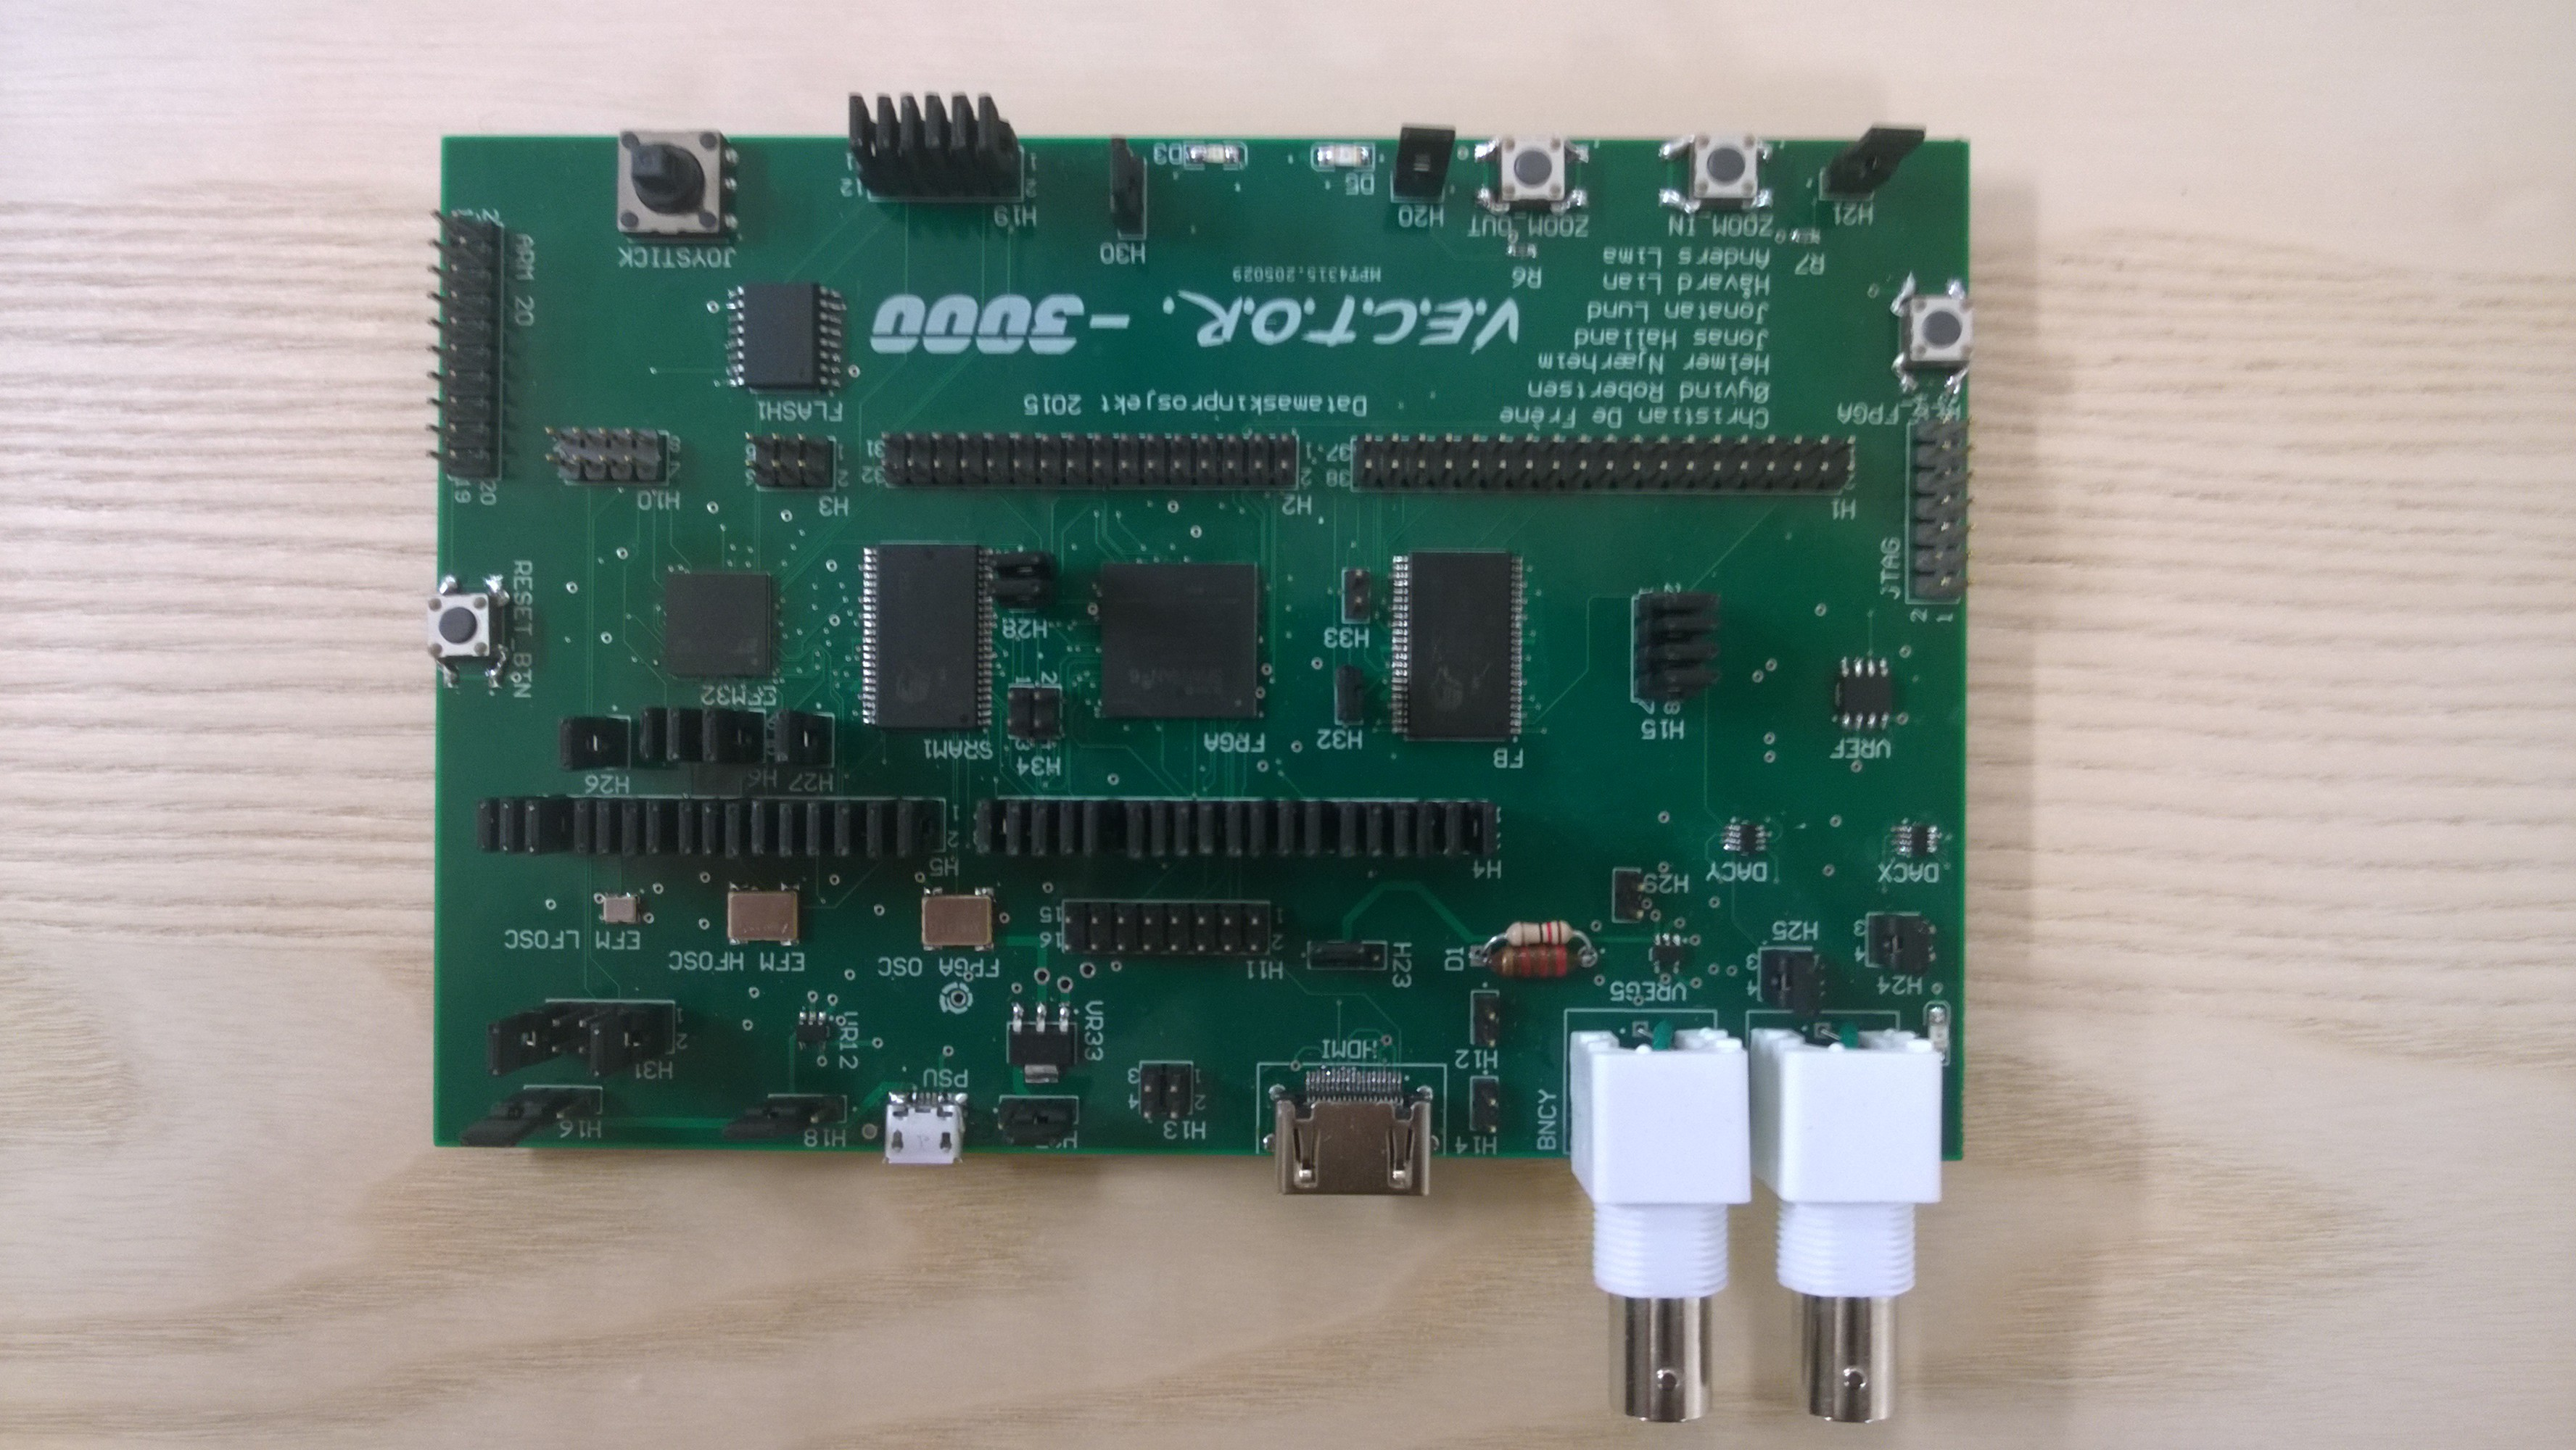
\includegraphics[width=\linewidth, angle=180]{images/board.jpg}
	    \caption{An image of the finished \vthreek board}
	    \label{fig:board}
\end{figure}

\section{Storage}
The final implementation utilizes BRAM to achieve highest possible clock frequency and avoid unnecessary SRAM access delays.
With the current implementation the BRAM can hold a total of 1024 primitives.
The synthesis report from Xilinx Ise states that the FPGA still has more BRAM after.
However the primitive storage space is not the limiting factor, but the primitive drawing module.

\section{Performance}
The maximum clock frequency of the DACs is 30MHz according to the datasheet.
To update the DAC value a total of 25 clock cycles are required.
As a result the theoretical effective maximum output will be \(30 MHz \div 25 = 1.2 MHz \).
However during testing the group experience incorrect DAC values if the clock were set higher than 20 MHz.
With a clock frequency of 20 MHz the maximum output is 800 KHz.

\section{Drawing Artifacts}
The oscillioscope used in this project supports x and y inputs.
When the oscillioscope is done drawing one primitive and moves to the next the electron beam i still drawing,
and weaker drawing lines may be visible.
In other words all shapes are drawn without "litfing the hand."
If one take a closer look at figure~\ref{fig:artifact}, the drawing artifacts are visible.
There are solutions to avoid the drawing artifacts, which is exlained in section \ref{discussion:artifacts}.


\begin{figure}[h]
	    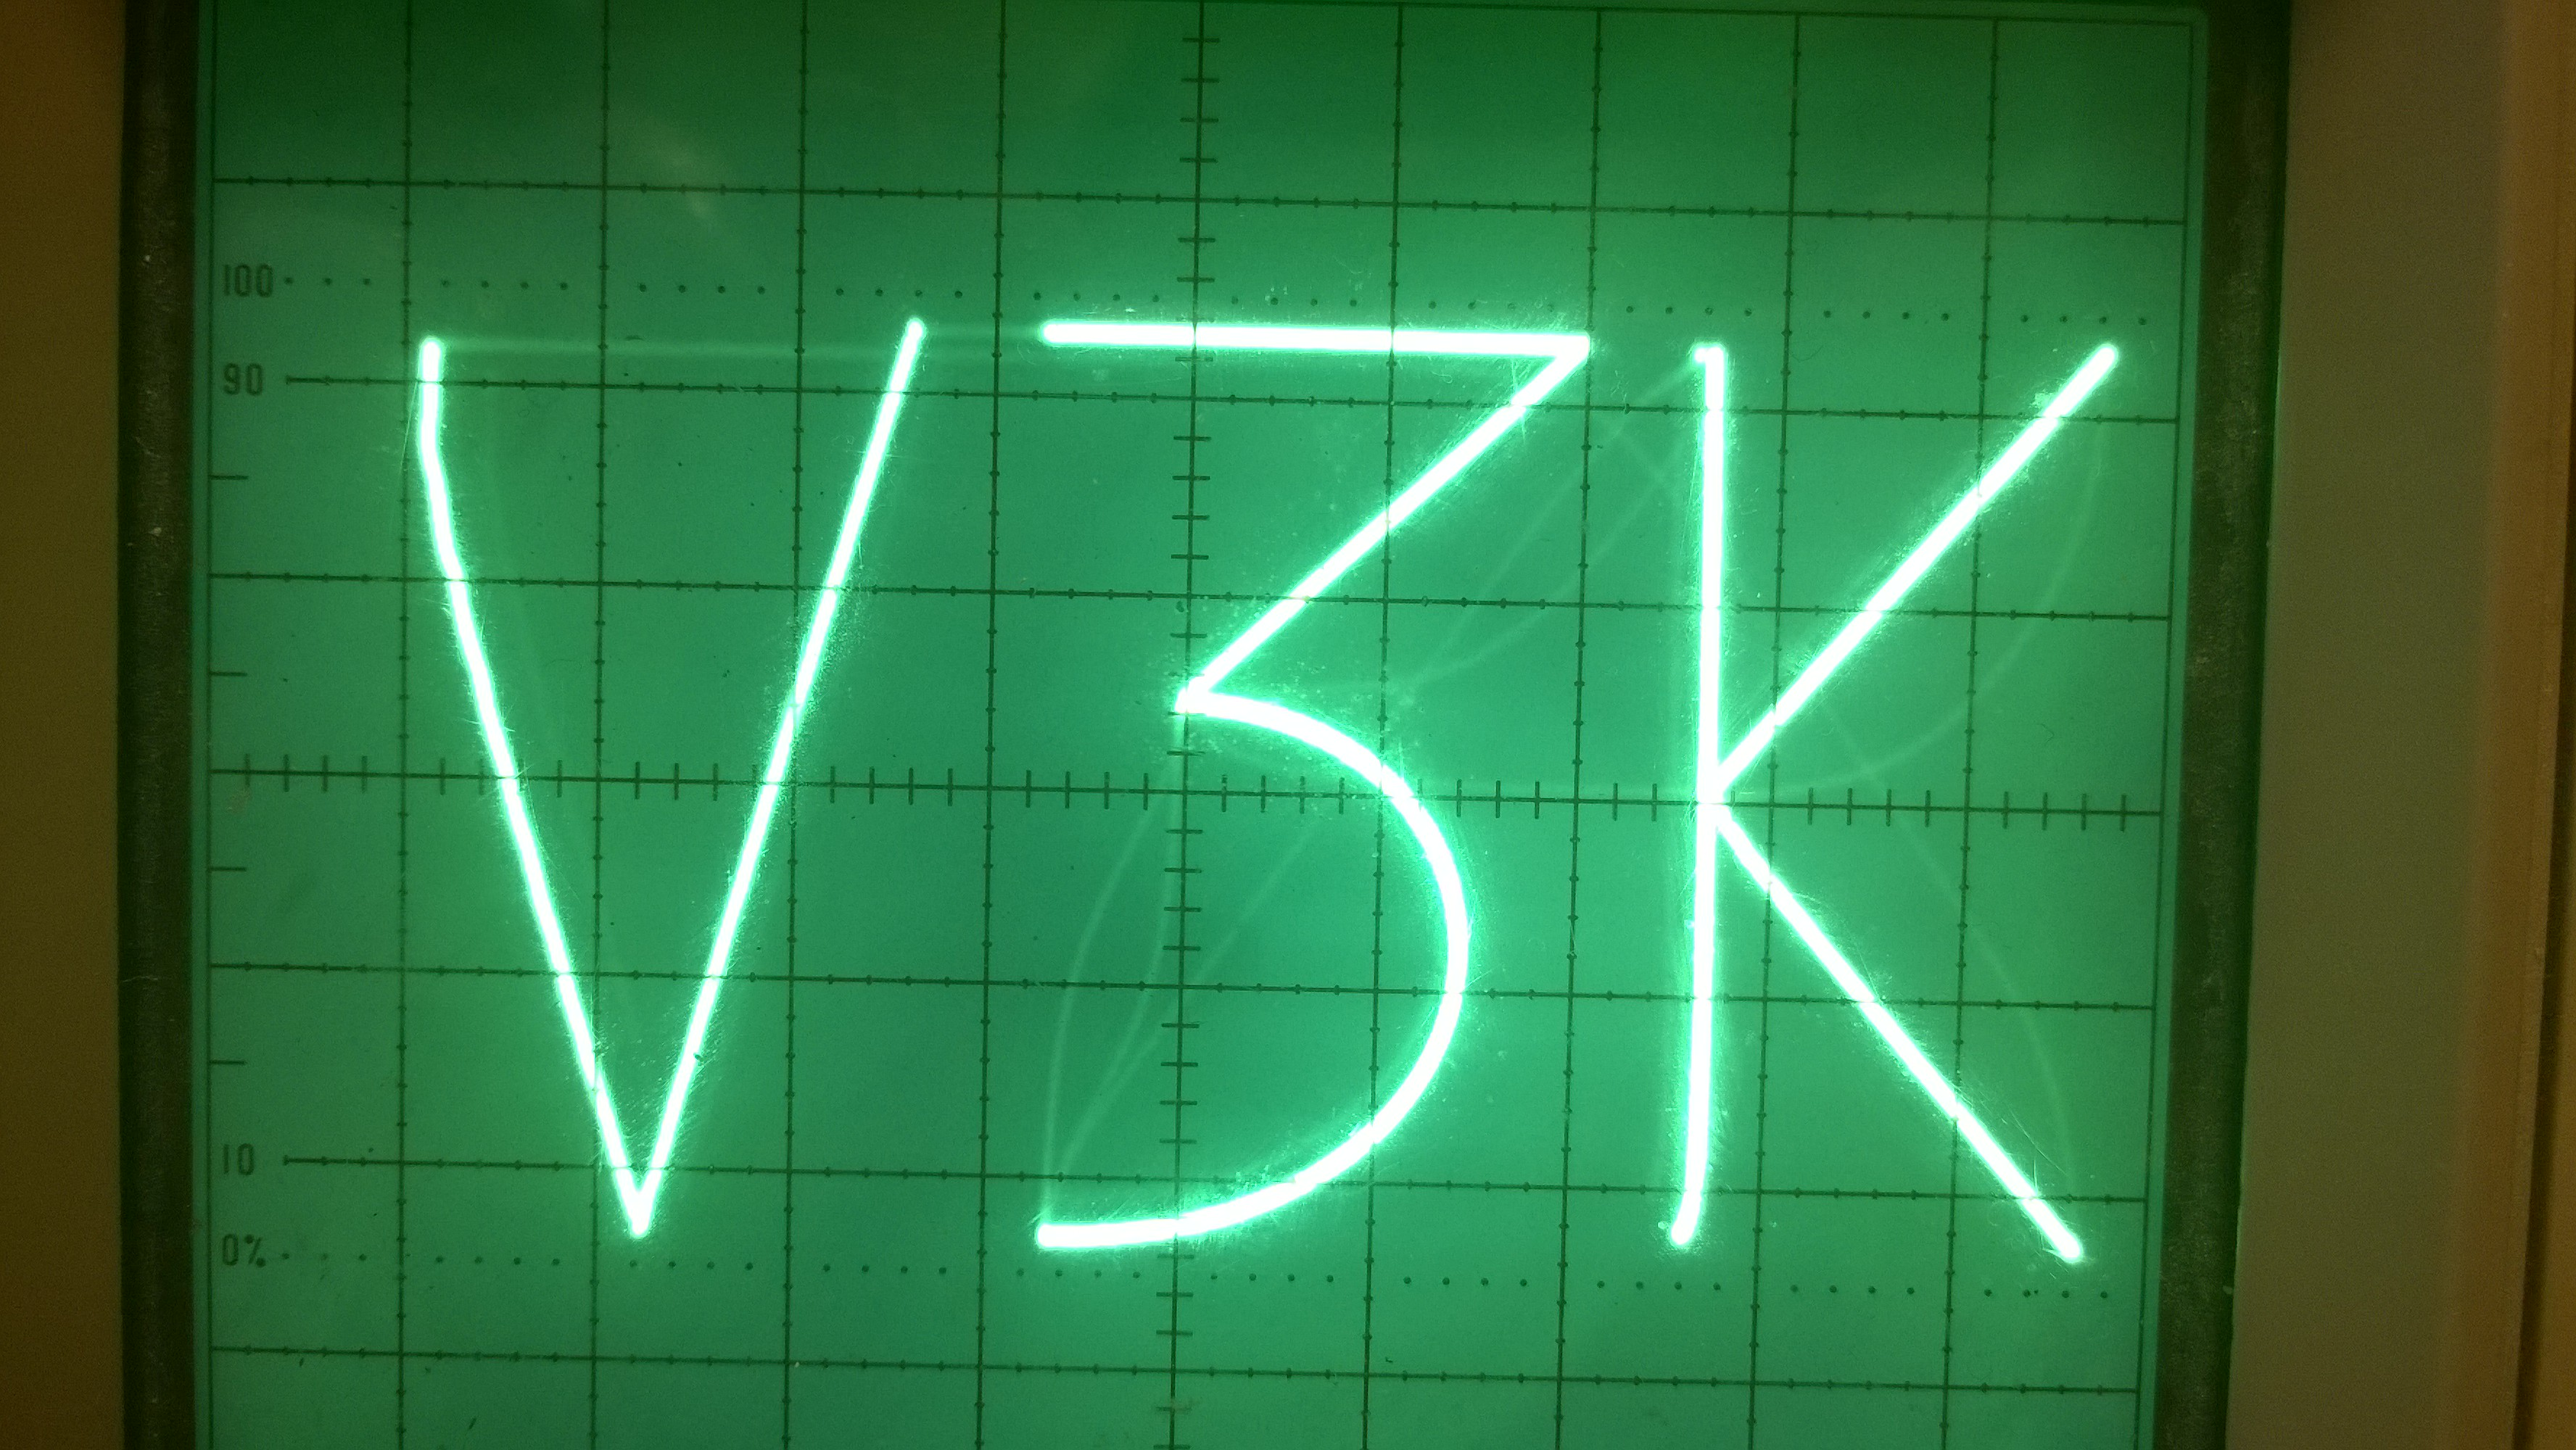
\includegraphics[width=\linewidth]{images/artifacts.jpg}
	    \caption{Drawing v3k with artifacts}
	    \label{fig:artifact}
\end{figure}
